% summerSHG - technical notes
% to be posted to the CGP logbook
% should contain: how TL works, characterisation of TL, jitter noise floor discussion
% should not contain: timeline or mistakes, just useful results and methodology (if pertinent to replication)

\documentclass[aps,pra,superscriptaddress,reprint,nofootinbib]{revtex4-1}
% \documentclass[prb,reprint,nofootinbib]{revtex4-1} 
% \documentclass[pra,superscriptaddress,reprint,nofootinbib]{revtex4-1}
% \documentclass[prb,preprint,letterpaper,noeprint,longbibliography,nodoi,footinbib]{revtex4-1} 

% worry about formatting AFTER the text is written

\usepackage[utf8]{inputenc}
\usepackage{amsmath,amssymb,amsthm}
\usepackage{amsfonts}
\usepackage{graphicx}
\usepackage{float}
\usepackage{mathtools}
\usepackage[usenames,dvipsnames]{xcolor}	
\usepackage{hyperref}
% \usepackage{siunitx}
\usepackage{textcomp}
% \usepackage{subfiles}
\usepackage{comment}
% \usepackage[bottom]{footmisc}
% \usepackage{subfig}
% \usepackage[style=base]{caption}
\usepackage[caption=false]{subfig}

\usepackage{silence}
\WarningFilter{revtex4-1}{Repair the float}

%\bibliographystyle{apsrev4-2}
%\setlength{\parindent}{0pt}

% \newcommand{\abs}[1]{\left\lvert #1 \right\rvert}
% \newcommand{\norm}[1]{\left\lVert #1 \right\rVert}
% \newcommand{\ip}[2]{\langle #1,#2 \rangle}
% \newcommand{\expect}[1]{\langle #1 \rangle}

% \newcommand{\code}[1]{\texttt{#1}}
% \newcommand{\jam}[1]{\textcolor{magenta}{\textbf{#1}}}


\begin{document}
\title{Tilt locking the OPO - Technical notes}

\author{James W. Gardner}
\email{u6069809@anu.edu.au}
\affiliation{Centre for Gravitational Astrophysics, The Australian National University, Acton, A.C.T., 2601, Australia}
\affiliation{OzGrav @ ANU, Australian Research Council Centre of Excellence for Gravitational Wave Discovery, Acton, A.C.T., 2601, Australia}

\author{Min Jet Yap}
% \email{vaishali.adya@anu.edu.au}
\affiliation{Centre for Gravitational Astrophysics, The Australian National University, Acton, A.C.T., 2601, Australia}
\affiliation{OzGrav @ ANU, Australian Research Council Centre of Excellence for Gravitational Wave Discovery, Acton, A.C.T., 2601, Australia}

% \author{David McClelland}
% % \email{david.mcclelland@anu.edu.au}
% \affiliation{Centre for Gravitational Astrophysics, The Australian National University, Acton, A.C.T., 2601, Australia}
% \affiliation{OzGrav @ ANU, Australian Research Council Centre of Excellence for Gravitational Wave Discovery, Acton, A.C.T., 2601, Australia}

% \author{Sheon Chua}
% % \email{vaishali.adya@anu.edu.au}
% \affiliation{Centre for Gravitational Astrophysics, The Australian National University, Acton, A.C.T., 2601, Australia}
% \affiliation{OzGrav @ ANU, Australian Research Council Centre of Excellence for Gravitational Wave Discovery, Acton, A.C.T., 2601, Australia}

\date{\today}


%%%%%%%%%%%%%%%%%%%%%%%%%%%%%%%%%%%%%%%%%%
% \begin{abstract}
% % single paragraph, short sales pitch
% \end{abstract}

\maketitle

%%%%%%%%%%%%%%%%%%%%%%%%%%%%%%%%%%%%%%%%%%
\tableofcontents

\section{Preamble}
\label{sec:preamble}

These notes are written as a technical reference for the CGA squeezer group and assume an appropriate level of familiarity with the squeezer OPO table and any relevant concepts. They are aimed at an audience interested in implementing tilt locking.
These notes do not give a chronological account of our work nor do they contain everything we attempted. For further information see the accompanying ``tilt locking'' series of posts in the CGP Logbook~\footnote{\url{http://chimera1.physics.anu.edu.au/wordpress/?tag=tilt-locking}} or contact the authors.

This work was done in the Summer of 2020/2021 as part of an internship with CGA.

\subsection{Content guide}

This Section~\ref{sec:preamble} describes what these notes contain and their purpose.
Section~\ref{sec:TL} motivates, explains, and details our implementation of tilt locking (TL).
Section~\ref{sec:error_signal} gives a guide to improving the error signal of the TL control system.
Section~\ref{sec:out-of-loop_sensors} motivates and details the out-of-loop sensors that we used to characterise the TL control system.
Section~\ref{sec:results} contains miscellaneous results that characterise the TL control system and compare its performance to the PDH control system previously implemented.
And Section~\ref{sec:conclusions} draws conclusions about the efficacy of the TL control system.


%%%%%%%%%%%%%%%%%%%%%%%%%%%%%%%%%%%%%%%%%%
\section{Tilt locking (TL)}
\label{sec:TL}

It should be noted that what we did with TL was not novel. Motivated by the reasons below, we were interested in investigating whether it, as a pre-existing technology, was right for our uses.

\subsection{Motivation}

For squeezing experiments down the beamline, we want to keep the OPO on resonance to maximise the laser power inside the cavity. Whether the cavity is on resonance (considering plane waves for the moment) depends on the laser frequency and the cavity tuning. Here, we are trying to lock the cavity length as to stay on resonance for the fundamental spatial mode~\footnote{Note that we will refer to cavity tuning interchangeably as cavity length throughout these notes which may be confusing if one insists that length be restricted to integer multiples of the carrier wavelength.}.


The OPO table already had a PDH control system in place to perform this function. One purpose of this work was to compare that existing system (PDH) to an alternative control system (tilt locking, see below). 


\subsection{Optics theory for TL}

This understanding and implementation are based on the work in Ref.~\cite{TL:1999}, see that reference for further information.


Classically, the laser light incident on the cavity can be decomposed into the Hermite-Gauss (HG) rectangular modes. How much the cavity is detuned determines how it ``sees'' these modes. Critically, the different spatial structure of these modes makes each acquire a different Gouy phase upon circulation. This implies a different resonance condition (length) for each mode. As such, at different detunings, the cavity will ``see'' different modes as resonant.


We restrict our attention to the fundamental (a single blob) and the first-order (two blobs side-by-side either vertically or horizontally along the two transverse x and y axes, respectively) HG modes. We placed a quadrature photodiode (QPD) to detect the light reflected off of the cavity such that the quadrature axes were (roughly) aligned with the horizontal and vertical transverse axes of the beam. The QPD outputs SUM, YDIFF, and XDIFF channels for the total intensity and the difference in intensity on the horizontal and vertical halves, respectively. If either mode is incident on the QPD alone, then the DIFF signals are zero (supposing that the beam is properly aligned). But if the fundamental and a first-order mode are both present at the QPD, then their interference can produce a non-zero DIFF signal for the relevant axis.


When the cavity is exactly on resonance for the fundamental, the error signal is still zero (see Ref.~\cite{TL:1999}). Then, when slightly off resonance, the DIFF signal response is approximately linear with the cavity tuning as the fundamental acquires extra phase but the higher-order mode does not. Tilt locking uses this linear response near the zero-crossing associated with the fundamental resonance as its error signal for controlling the cavity length by driving a PZT behind one of the cavity mirrors.


\subsection{Implementation}

\begin{figure*}
	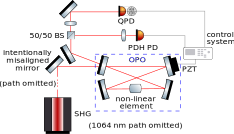
\includegraphics[height=0.6\textwidth,angle=-90]{figures/TL_layout.pdf}
	\caption{Schematic for tilt lock layout for cavity length control with PDH as an out-of-loop sensor.}
	\label{fig:TL_layout}
\end{figure*}

As of the time of writing, the TL set-up is as displayed in Fig.~\ref{fig:TL_layout}. The path from the SHG to the OPO was unchanged except for intentional misalignment of the final steering mirror into the cavity (see Sec.~\ref{sec:misalignment}). The bow-tie cavity of the OPO was similarly unchanged (and we used the same PZT for both control systems). The reflected field from the cavity passes through a lens and a dichroic mirror (neither shown in Fig.~\ref{fig:TL_layout}) to send the 1064 nm squeezed vacuum down-line. Apart from the above-mentioned misalignment, our implementation only changed the path for the 532 nm which previously went to a PD for PDH control of the cavity length. Now, the beam hits a 50/50 beamsplitter to split to the relocated PDH system (for out-of-loop monitoring, see Sec.~\ref{sec:PDH_out-of-loop}) and the new TL path.

The TL path consists of a 50~mm lens (placed far back from the QPD to increase the spot size, see Sec.~\ref{sec:spot_size}), a mirror, and the QPD explained above. The lens was placed before the QPD steering mirror to avoid unpredictable behaviour (previously, the placement was such that we had to hit the edge of the lens to steer onto the QPD). We aligned the TL system by steering the beam through the centres of all of the optics and visually onto the PD. Then, we tried to get the DC offset of the YDIFF and XDIFF signals to be zero while maximising the SUM signal, as that would indicate hitting the centre of the crosshair (assuming that the PD response was uniform across the face of the QPD).

For electronics, we used the existing servo and HV amp eurocards from the PDH control system to drive the PZT. For TL, the YDIFF signal was the positive input into the servo, its positive output was fed to the HV amp, and the amp output was sent to the PZT.

Throughout we used a DSO-X 3034A oscilloscope for monitoring and an SR785 spectrum analyser for LF (below 100~kHz) measurements. All of the Python 3 Jupyter notebooks~\cite{python,ipython,jupyter} we used to plot and analyse the data are collected and commented in a GitHub repository~\footnote{\url{https://github.com/daccordeon/summerSHG}}.


\subsection{Achieving lock}

To achieve lock the system must be manually guided to the linear regime of the YDIFF error signal by use of the DC offset knob on the servo panel (so-called “manual lock acquisition”). Monitoring the QPD SUM and YDIFF signals on the oscilloscope, the user must slowly change the DC offset until the QPD SUM dips down and the error signal nears zero (signs of nearing a resonance). Then, quickly, the user must switch on the proportional (labelled as “signal”) and integral control. If the lock is successful, then the YDIFF error signal should remain at zero and the SUM should stay down. One can then create a disturbance (e.g.\ by clapping, stomping, or talking near the optics table) and see that the system maintain lock. 


Likely, the lock will not be initially achieved. The YDIFF error signal may need to be improved by the methods detailed in Sec.~\ref{sec:error_signal}, below. Alternatively, the servo gain may be too low and should be increased. If failure to lock is due to the lock finding the high-order resonance instead of the fundamental, then the user must reset and try again. If the system appears to be ringing while in lock or is losing lock due to ringing, then the servo gain should be turned down.


%%%%%%%%%%%%%%%%%%%%%%%%%%%%%%%%%%%%%%%%%%
\section{Improving the error signal}
\label{sec:error_signal}

In this Section, we outline (some of) the noise sources for the TL and some methods of improving the YDIFF error signal that we tried.

\subsection{QPD dark noise and jitter noise}

The QPD has dark noise: noise present in its output even when no laser light and minimal environmental light is incident on it. This dark noise was a benchmark for the TL control system to get down to and was later compared to the PDH dark noise (as dark noise cannot be removed, only reduced with better electronics, they represent limits for each control system). We measured the dark noise by blocking the beam before the OPO and measuring the YDIFF output with the lid on the optical table.

Because we are monitoring the difference in intensities incident on different quadratures, the TL system is sensitive to jitter noise: noise from the thermal, seismic, and sonic sources that shake the various optics along the beam path before the QPD and steer the beam spot off-centre to erroneously give a DIFF signal even with, for example, only the fundamental HG mode present. The jitter noise is affected by the path length to reach the QPD (the spatial misalignment increases the further the beam travels) and the quietness of the surrounding environment. We measured the jitter noise by blocking the beam inside the OPO behind the first mirror, this eliminates any cavity effects to produce the higher-order HG modes and so we just see the motion of the optics.

The QPD jitter noise was measured between a factor of two and an order above its dark noise but seemed to vary between days (source unknown), see Sec.~\ref{sec:jitter_sensor_noise}.

\subsubsection{Other electronic dark noise}

We also checked the SR785’s electronic dark noise floor and found it at least an order below the QPD’s dark noise. As such, we ignored it from then on and refer to only the photodiode(s) when we refer to dark noise, henceforth.

\subsection{Intentional misalignment into the cavity}
\label{sec:misalignment}

\begin{figure}
\includegraphics[width=0.4\textwidth,angle=-180]{figures/20201222_114552_error_sig.jpg}
\caption{Oscilloscope measurement from 2020-12-22. The TL YDIFF error signal (red), the QPD SUM (yellow), and the ramp scan (blue).}
\label{fig:TL_error_sig_example}
\end{figure}

The TL YDIFF error signal can be seen by scanning the cavity using a 6~Hz, -1~V to 4~V ramp. An example is shown in Fig.~\ref{fig:TL_error_sig_example}. The best method we found was to introduce a horizontal misalignment at the last steering mirror into the cavity, shown in Fig.~\ref{fig:TL_layout}. This moved the zero-crossing of the error signal closer to the fundamental resonance and kept a large linear region on either side. However, the misalignment should not be so great as to significantly increase the first-order mode resonance peak in the QPD SUM channel (introducing misalignment into the cavity makes the cavity ``see'' more of the higher-order mode). If over-done, then the control system is more likely to lock to the wrong resonance peak.

We found that introducing a small misalignment was all we needed to improve the slope around the zero-crossing (the error signal should be monitored as it changes shape).

\subsection{Putting the lid on the optical table}

\begin{figure}
\includegraphics[width=0.45\textwidth]{figures/20201221_114754_lid_on.jpg}
\caption{SR785 measurement from 2020-12-21 of YDIFF and XDIFF dark noise with the optical table lid on and off.}
\label{fig:dark_noise_lid_on}
\end{figure}

To improve the dark noise, we put the lid on the optical table to reduce the amount of environmental light incident on the QPD. This improved the dark noise at LF by at least two orders, as seen in Fig.~\ref{fig:dark_noise_lid_on}. Therefore, we put the lid on the optical table for all other measurements.

\subsection{Increasing the spot size}
\label{sec:spot_size}

We also tried increasing the beam spot size incident on the QPD to increase the sensitivity of the TL system. We thought that a larger spot size would lie across multiple quadrants and so detect changes that a beam restricted to one quadrant could not. We did this by including a converging lens before the QPD but beyond its focal length so that the beam was diverging for long enough to increase the spot size. Note that we included the lens before the TL steering mirror for ease of alignment since the position of the QPD on the stand meant that, otherwise, we would have to steer through the edge of the lens, which is not ideal.

Including the lens increased the slope of the error signal and so the sensitivity by around a factor of two, comparing the traces in the relevant logbook post~\footnote{\url{http://chimera1.physics.anu.edu.au/wordpress/?p=15993}}. However, the misalignment was more effective at improving the error signal as it also moved the zero-crossing (it changes the shape of the error signal).


%%%%%%%%%%%%%%%%%%%%%%%%%%%%%%%%%%%%%%%%%%
\section{Out-of-loop sensors}
\label{sec:out-of-loop_sensors}

To characterise the TL control system, we introduced out-of-loop sensors to monitor the system.

\subsection{Control theory of sensor noise}

\begin{figure}
	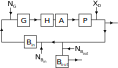
\includegraphics[height=0.4\textwidth,angle=-90]{figures/FCS_diagram.pdf}
	\caption{Block diagram for a SISO feedback control system with an out-of-loop sensor, $B_{\mathrm{out}}$. $B_{\mathrm{in}}$ is the in-loop sensor, $G$ is the compensator, $H$ is the driver, $A$ is the actuator, $P$ is the plant. The disturbance upon the free-running variable is $X_d$, the sensor noises are $N_{B_{i,o}}$, and the compensator noise is $N_G$.}
	\label{fig:block_FCS_diagram}
\end{figure}


This understanding is based on the introduction to control theory provided by Refs.~\cite{Ward:2010,Bechhoefer:2005,FCS:2000}.


Consider a simple SISO (single-input single-output) feedback loop, shown in Fig.~\ref{fig:block_FCS_diagram}, working to suppress the disturbance to some variable in the system (as opposed to tracking a reference signal). The sensor observes the variable and produces an error signal for the compensator, which commands the driver-actuator to act on the plant as to make the error signal zero. Noise enters the system at three points: the free-running disturbance to the variable after the plant, the sensor, and the compensator. Note that while, a priori, noise could enter elsewhere in the system, these are assumed to be the dominant sources~\cite{FCS:2000}. 


The free-running disturbance is suppressed at the control output (the signal input to the sensor) by the open-loop gain. If the gain is high enough such that the noise at the sensor (which does not change with gain) becomes dominant, then the sensor will start (unknowingly) treating it as a true disturbance to the system and will cause the plant to act on the system as to counter it, thereby introducing so-called ``sensor noise'' into the system that the control loop is meant to be quieting. Further increasing the gain only injects more of this noise into the system. Sensor noise represents a limit to the efficacy of a control system since the sensor cannot distinguish its noise from that in the physical system.


The tricky part of sensor noise, however, is that at the sensor output it is suppressed by the open-loop gain. This means that it will be suppressed in any data using the sensor itself. To solve this and observe the sensor noise, a second, out-of-loop, sensor is added to complement the existing in-loop sensor. This out-of-loop sensor is only used for monitoring the system and its error signal is not fed back to any control system. Supposing that the out-of-loop sensor’s noise is not louder than the in-loop sensor’s noise, then in regions of high gain where sensor noise is injected into the system the error signal from the out-of-loop sensor should hit a noise floor that cannot be passed by increasing gain. Meanwhile, the in-loop sensor would erroneously show better and better error signals.


\subsection{XDIFF}

\begin{figure*}
\includegraphics[width=0.7\textwidth]{figures/TL_residual_error_full_spectrum_comparison_no_bands.pdf}
\caption{SR785 measurements from 2020-12-23 of the TL YDIFF residual error (blue) compared against dark noise (orange) and jitter noise (green).}
\label{fig:TL_residual_error_full_spectrum_comparison_no_bands}
\end{figure*}

\begin{figure*}
\includegraphics[width=0.7\textwidth]{figures/TL_XDIFF_and_YDIFF_spectra_comparison.pdf}
\caption{SR785 measurements from 2021-01-06 comparing the XDIFF and YDIFF residual errors against their dark noises while TL’d against YDIFF. We see that YDIFF goes below dark noise below 10~Hz but that XDIFF remains above dark noise throughout. The residual errors are normalised to the gradient at the zero-crossing in the scanned cavity error signal, i.e.\ normalised to the sensitivity of each sensor, but the dark noise measurements are not normalised.}
\label{fig:TL_XDIFF_and_YDIFF_spectra_comparison}
\end{figure*}

We decided to implement an out-of-loop sensor because the TL residual error (the error signal with lock acquired) was measured to be below its dark noise (and the jitter noise) below 10~Hz, seen in Fig.~\ref{fig:TL_residual_error_full_spectrum_comparison_no_bands}. These are sources of noise for the QPD YDIFF in-loop sensor and so we wanted to observe the sensor noise in an out-of-loop sensor.

We initially used the XDIFF (vertical) signal as an out-of-loop sensor~\footnote{There is no preference for horizontal over vertical spatial alignment, if XDIFF is used for control, then YDIFF could be used for monitoring.}. This meant that we also measured the XDIFF channel whenever taking readings and so required no changes to the existing implementation beyond some vertical misalignment into the cavity to improve the XDIFF error signal as to detect changes to the cavity length.

We then TL’d (tilt locked) the OPO and observed that the XDIFF out-of-loop sensor was above its dark noise, as seen in Fig.~\ref{fig:TL_XDIFF_and_YDIFF_spectra_comparison}. We normalised each sensor to its error signal’s slope at the zero-crossing near the fundamental resonance (a measure of its sensitivity). For later measurements, we used this slope to convert to length noise, see Sec.~\ref{sec:length_noise}.

In retrospect, the XDIFF signal was likely at a noise floor determined by its vertical jitter noise plus some amount of jitter sensor noise from the control system. However, we only investigated this further with the other out-of-loop sensor that we tried (see \ref{sec:jitter_sensor_noise}).


\subsection{PDH}
\label{sec:PDH_out-of-loop}

\begin{figure*}
    \subfloat[\centering]{{	\includegraphics[width=0.5\textwidth]{figures/TL_dark_noise_comparison_to_PDH.pdf}}}%
    \subfloat[\centering ]{{\includegraphics[width=0.5\textwidth]{figures/TL_dark_noise_comparison_to_PDH_new_mixer.pdf}}}%
	\caption{SR785 measurements from 2021-01-13/14 of the TL and PDH dark noise. Showing PDH dark noise from the old eurocard mixer (panel a, left) and from the new mixer (panel b, right). The new mixer flattens the PDH dark noise and brings it under TL at LF.}
	\label{fig:TL_dark_noise_comparison_to_PDH}
\end{figure*}

We stopped using the XDIFF channel as the out-of-loop sensor to compare the efficacy of the TL control system against PDH~\footnote{The reader is expected to already understand the mechanism of PDH control for cavity length.}. To use PDH as the out-of-loop sensor, we included it in the other beam path after the 50/50 beamsplitter, as shown in Fig.~\ref{fig:block_FCS_diagram}.

Initially, the PDH had too much attenuation to see anything other than its dark noise, so some attenuation was removed. Then, we were surprised at the features in the PDH dark noise and that it was higher than the TL dark noise, shown in the left panel of Fig.~\ref{fig:TL_dark_noise_comparison_to_PDH}. We tracked this down to the old mixer eurocard used. We replaced it with a Minicircuits ZP-3+ with an attached LP filter, which improved and flattened the dark noise and also allowed for some attenuation to be removed which further improved the SNR, shown in the right panel of Fig.~\ref{fig:TL_dark_noise_comparison_to_PDH}.

The latter dark noise measurement allows for an early conclusion to be made about the efficacy of TL compared to PDH. If we assume that there are no other noise sources, then each will be limited by its dark noise and so PDH will outperform TL at LF (below 1~kHz) and TL will outperform PDH between 1~kHz and 100~kHz (unless the peaks there are relevant).


%%%%%%%%%%%%%%%%%%%%%%%%%%%%%%%%%%%%%%%%%%
\section{Results}
\label{sec:results}

In this section, we characterise the TL control system and compare its performance to PDH.

\subsection{Open-loop gain}
\label{sec:OLG}

\begin{figure*}
	\includegraphics[width=0.8\textwidth]{figures/TL_OLG_and_CLG.pdf}
	\caption{SR785 measurements from 2021-01-05 of Bode amplitude and phase for the transfer function of the TL control system (i.e.\ the OLG) with 10~mV swept sine injected after the in-loop sensor. Also showing the closed-loop gain calculated as $\mathrm{CLG} = \frac{1}{1+\mathrm{OLG}}$ and the unity-gain frequency (UGF) where the gain is 0~dB. The phase measurements are relative to $-180^\circ$.}
	\label{fig:TL_OLG_and_CLG}
\end{figure*}

To characterise the TL, we measured the open-loop gain (OLG) of the system. This is detailed in the relevant post in the CGP logbook~\footnote{\url{http://chimera1.physics.anu.edu.au/wordpress/?p=16025}}. A swept sine measurement from the SR785 was injected by an adder board after the in-loop sensor and the ratio of the signals at two test-points, before and after the injection of the external signal, was measured and is shown in Fig.~\ref{fig:TL_OLG_and_CLG}. We also calculated the closed-loop gain as $\frac{1}{1+\mathrm{OLG}}$ since the control system is operating in a disturbance-suppression mode~\cite{FCS:2000}.

We measured the unity-gain frequency (UGF) to be around 8-12~kHz and can see that the system is stable, given the Nyquist criterion, with high phase margin but low gain margin. Below the UGF, the system falls as 20~dB over one order of magnitude in frequency and the phase sits around $90^\circ$ away from $-180^\circ$, indicating a 1/f gain at LF, consistent with the Bode gain-phase relation. Above the UGF, the system shows resonances but is made stable by the 10~Hz low-pass filter in the HV amp which also allows for a higher UGF, see the explanation in the logbook post.

\subsubsection{Measuring the servo gain}

For reference, we also wanted to know the gain across the servo. We did this by injecting a 6~Hz, 30~mV peak-to-peak sine signal into the servo without adjusting the gain knob (or rather, taking great care not to). Then, we measured the peak-to-peak of the output on the oscilloscope to calculate the servo gain.

\subsection{Calibrating length noise}
\label{sec:length_noise}

\begin{figure}
	\includegraphics[width=0.5\textwidth]{figures/TL_and_PDH_length_scan_2021-01-20.pdf}
	\caption{Oscilloscope measurements from 2021-01-20 of TL and PDH error signals from a ramp scan of the cavity. Also showing slope fits around the zero-crossing near the fundamental resonance. The horizontal axis has been calibrated from time to length by using the spacing of the fundamental resonances in the QPD SUM data (not shown) and assuming that the laser frequency is 532 nm.}
	\label{fig:TL_and_PDH_length_scan_2021-01-20}
\end{figure}

Considering the system abstractly, as in Fig.~\ref{fig:block_FCS_diagram}, the in and out-of-loop sensor outputs are not directly comparable as they are in different parts of the block diagram. To properly compare, say, the TL jitter noise and the PDH residual error we need to project the signals back before their respective sensors into the common variable of the cavity length~\footnote{The problem is not that the sensor outputs do not have the same dimensions, but that they may have been scaled by different values by the different sensors.}.

To invert the effect of the sensors, we normalise the DC voltage (that acts as a scalar gain) and calibrate into length. We do so using the slope of the error signal at the zero-crossing near the fundamental resonance, measured from scanning the cavity with a 6~Hz, -1 V to 4 V peak-to-peak ramp and shown in Fig.~\ref{fig:TL_and_PDH_length_scan_2021-01-20}. Dividing the sensor output (in volts) by the slope (in volts per metre) gives the length noise (in metres), which we can then compare between the two.


\subsection{Jitter sensor noise}
\label{sec:jitter_sensor_noise}

\begin{figure*}
	\includegraphics[width=0.8\textwidth]{figures/TL_length_noise_compared_to_PDH_length_noise_floor.pdf}
	\caption{SR785 LF measurements from January 2021 of TL and PDH dark and jitter noise projected into length noise using the error signal slopes. Comparing to projected PDH residual error noise floor at high gain, with normalised DC voltage.}
	\label{fig:TL_length_noise_compared_to_PDH_length_noise_floor}
\end{figure*}

With the TL at high gain such that its residual error was below its dark and jitter noise, we measured the PDH residual error and compared it against the predicted jitter sensor noise floor, shown in Fig.~\ref{fig:TL_length_noise_compared_to_PDH_length_noise_floor}. We see that the PDH residual error is comparable to and appears limited by the TL jitter length noise across all frequencies, as predicted. We also see that PDH itself is not affected directly by jitter noise, which makes sense as it is not spatial.

\subsubsection{Complications}

\begin{figure*}
	\includegraphics[width=0.8\textwidth]{figures/TL_and_PDH_TLd_residual_errors_two_gains.pdf}
	\caption{SR785 LF measurements from 2021-01-20 of TL and PDH dark and jitter noise projected into length noise. Compared against high and low gain residual errors. Note that this data was taken after that in shown in Fig.~\ref{fig:TL_length_noise_compared_to_PDH_length_noise_floor}.}
	\label{fig:TL_and_PDH_TLd_residual_errors_two_gains}
\end{figure*}

We also investigated the effect of servo gain on the out-of-loop sensor, shown in Fig.~\ref{fig:TL_and_PDH_TLd_residual_errors_two_gains} for a low gain that barely kept the system in lock and a high gain just below where the system started noticeably ringing. At low gain, the two residual errors agree and are far above the jitter and dark noise floors, as expected when the laser is on and the actuator is weakly driven. At high gain, the TL residual error dips below its dark noise but the PDH residual error does not reach the jitter noise, which itself has dropped and is far less than an order above the dark noise, unlike the data in Fig.~\ref{fig:TL_length_noise_compared_to_PDH_length_noise_floor}.

The reason for the decrease in jitter noise compared to the above measurements (i.e.\ comparing Fig.~\ref{fig:TL_and_PDH_TLd_residual_errors_two_gains} to Fig.~\ref{fig:TL_length_noise_compared_to_PDH_length_noise_floor}) is unknown. Similarly, what noise floor above the projected jitter noise that the PDH has reached is unknown (it could be sensor noise from the TL or something directly affecting the PDH). That the jitter noise appears to be different between days and that some unknown noise source is in the system are both curious observations.


%%%%%%%%%%%%%%%%%%%%%%%%%%%%%%%%%%%%%%%%%%
\section{Conclusions}
\label{sec:conclusions}

We have successfully implemented TL with minimal set-up and have characterised it as a control system by measuring its open-loop gain and by using PDH as an out-of-loop sensor. From the results in Sec.~\ref{sec:jitter_sensor_noise}, we see that jitter sensor noise is limiting the control system (although some complications remain unsolved). We also know that jitter noise and TL dark noise are above, sometimes by an order or more, the PDH dark noise (comparing all as length noise).
Therefore, if jitter noise is not reduced, then TL is stuck at a noise floor at least an order above PDH dark noise at LF, making it an inferior control system in its ability to quiet the cavity~\footnote{We have ignored noise sources for PDH other than its dark noise, in reality, PDH may not reach its dark noise.}~\footnote{This is a reductionist view of comparing the two systems, really, we should compare them across all frequencies below their UGF’s and also consider their stability, etc. Ref.~\cite{FCS:2000} gives a guide to designing control systems and how to decide on what sensors to use.}.

\subsection{Advice to those in the future}

If TL was to be used in the future, then the following problems should be considered: 
\begin{enumerate}
\item How should jitter noise be reduced?
	\begin{enumerate}
	\item How can the beam path be kept as short as possible (spatial misalignment grows over distance)?
	\item Can the system be better seismically isolated (seismic noise)?
	\item Can the system be cooled (thermal noise)?
	\item Can the system be placed in a vacuum (gas noise)?
	\item Why is the jitter noise time-varying?
	\end{enumerate}
\item Are a UGF of around 8-12~kHz and a maximum servo gain of around 67 sufficient to quiet the OPO (i.e.\ is length noise on the order of pm sufficiently small)?
\item Is TL stable enough at those high gains (recall that the phase margin is large but the gain margin is small)?
\item Is the PZT actuator range sufficiently large (a problem common to the current implementations of PDH and TL)?
	\begin{enumerate}
	\item Should a parallel laser frequency actuator be included in the control system?
	\end{enumerate}
\end{enumerate}

\section{Acknowledgements}

The authors would like to thank the CGA squeezer group, in particular Sheon Chua and Vaishali Adya, for their support and advice during the work.


%%%%%%%%%%%%%%%%%%%%%%%%%%%%%%%%%%%%%%%%%%
\nocite{*}
\bibliographystyle{myunsrt}
\bibliography{technical_notes}


\end{document}
